\documentclass[./main]{subfiles}

\begin{document}
  \chapter{Échauffement : deux algorithmes probabilistes.}

  \begin{exm}[Vérifier la multiplication de matrices]
    Soient $A, B, C$ trois matrices carrées à coefficients dans $\mathds{F}_2 = \{0,1\}$.
    On cherche à décider $AB = C$.

    \begin{description}
      \item[Idée 1.]
        On calcule $AB$ et on vérifie l'égalité à $C$.
        L'algorithme pour calculer $AB$ avec $(AB)_{i,j} = \sum_{k = 1}^n A_{i,k} B_{k,j}$ se fait avec une complexité en $\mathrm{O}(n^3)$.

        On peut améliorer la complexité en $\mathrm{O}(n^\alpha)$ avec $2 < \alpha < 3$ (actuellement, on peut le faire avec $\alpha \approx 2{,}37$) à l'aide de la méthode de Strassen.

      \item[Idée 2.]
        On calcule $ABx$ et $Cx$ pour un vecteur  $x \in \mathds{F}_2^n$.
        On a des multiplications $\text{matrices} \times \text{vecteurs}$, en complexité en~$\mathrm{O}(n^2)$.
        Pour trouver un "bon" vecteur $x$, on le choisit au hasard.
    \end{description}
    \label{exm:chap0-exm1}
  \end{exm}

  \begin{lem}
    Si $D \in \mathcal{M}_n(\mathds{F}_2)$ est non-nulle et $x \in \mathds{F}_2^n$ est choisi uniformément au hasard, alors on a $\mathrm{P}(Dx \neq 0) \ge \frac{1}{2}$.
  \end{lem}
  \begin{prv}
    Au moins un coefficient de $D$ est non-nul et, sans perte de généralité, on peut supposer que $D_{1,n} \neq 0$.
    Alors, 
    \[
      (Dx)_1 = \sum_{i=1}^n D_{1,i} x_i = \sum_{i=1}^{n-1} D_{1,i} x_i + x_{1}
    .\] 
    Quels que soient $x_1, \ldots, x_{n-1}$, il y a une probabilité de $\frac{1}{2}$ que $(Dx)_1 \neq 0$.
    On en conclut que \[ \mathrm{P}(Dx \neq 0) \ge  \mathrm{P}((Dx)_1 \neq 0) = \frac{1}{2}. \]
  \end{prv}

  \begin{exm}[suite de~\ref{exm:chap0-exm1}]
    Ainsi, si $AB \neq C$, on a donc \[\mathrm{P}(AB x \neq Cx) \ge \frac{1}{2}. \]

    On choisit $x_1, \ldots, x_{100}$ des vecteurs uniformément dans~$\mathds{F}_2^n$.
    Si on a $AB \neq C$, alors \[
    \mathrm{P}(\forall i \in \llbracket 1,100\rrbracket, ABx_i = Cx_i) \le \left(\frac{1}{2}\right)^{100}
    .\]

    On a donc un algorithme ayant une complexité $\mathrm{O}(n^2)$ pour détecter, avec grande probabilité, si $AB = C$.
  \end{exm}

  \begin{exm}[Coupe minimale dans un graphe]
    \label{exm:chap0-exm2}
    On considère $G$ un graphe non-orienté sans boucle (éventuellement avec des arêtes multiples).
    Une \textit{coupe} du graphe est un sous-ensemble $C \subseteq E$ tel que $(V, E \setminus C)$ n'est pas connexe.
    On cherche une coupe de taille minimale :
    \[
    \mathsf{mincut}(G) = \min \{|C|  \mid C \text{ est une coupe}\} 
    .\]

    De manière équivalente, on cherche une partition $V = V_1 \sqcup V_2$ (avec $V_1, V_2 \neq \emptyset$) qui minimise le nombre d'arêtes reliant $V_1$ et~$V_2$.

    Étant donné un graphe $G = (V, E)$, et une arête  $e = \{x,y\} \in E$, la \textit{contraction de $G$ selon $e$}, notée $G / e$, est le graphe où les sommets $x$ et $y$ sont fusionnés en un sommet $xy$, et les arêtes $\{x,z\}$ ou $\{y,z\}$ sont remplacées en $\{xy, z\}$ si $z \not\in  \{x,y\}$.

    \begin{figure}[H]
      \centering
      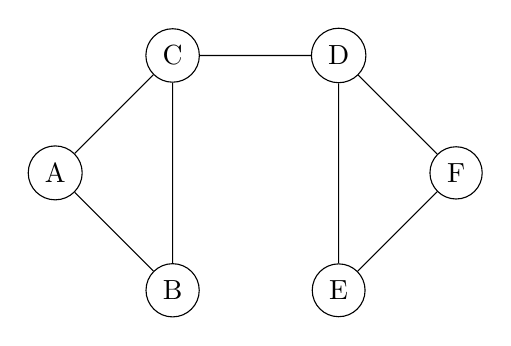
\begin{tikzpicture}[node distance=60]
        \node[draw, circle] (a) {A};
        \node[draw, circle, below right of=a] (b) {B};
        \node[draw, circle, above right of=a] (c) {C};
        \node[draw, circle, right of=c] (d) {D};
        \node[draw, circle, below right of=d] (f) {F};
        \node[draw, circle, below left of=f] (e) {E};
        \draw (a) -- (c) -- (b) -- (a);
        \draw (c) -- (d) -- (f) -- (e) -- (d);
      \end{tikzpicture}
      \[
      \vertical\longrightarrow
      \]
      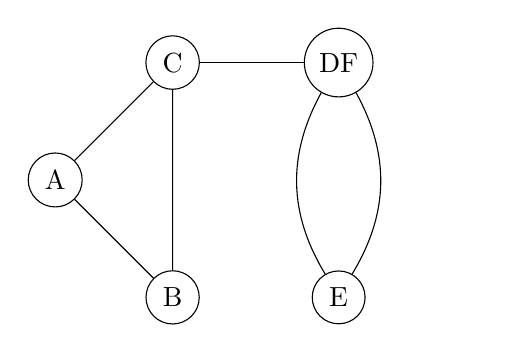
\begin{tikzpicture}[node distance=60]
        \node[draw, circle] (a) {A};
        \node[draw, circle, below right of=a] (b) {B};
        \node[draw, circle, above right of=a] (c) {C};
        \node[draw, circle, right of=c] (d) {DF};
        \node[draw, transparent, circle, below right of=d] (f) {F};
        \node[draw, circle, below left of=f] (e) {E};
        \draw (a) -- (c) -- (b) -- (a);
        \draw (c) -- (d);
        \draw (d) to[bend left] (e);
        \draw (d) to[bend right] (e);
      \end{tikzpicture}
      \caption{Contraction de l'arête $\{\mathrm{D}, \mathrm{F}\}$.}
    \end{figure}

    On a que $\mathsf{mincut}(G / e) \ge \mathsf{mincut}(G)$.

    On utilise l'\textit{algorithme de Krager} (1993).
    On contracte successivement selon des arêtes choisies uniformément au hasard, jusqu'à n'obtenir que $2$ sommets, ce qui donne une coupe du graphe initial.
  \end{exm}

  \begin{lem}
    La coupe $C$ produite par l'algorithme de vérifie 
    \[
    \mathrm{P}(|C| = \mathsf{mincut}(G)) \ge \frac{2}{n^2}
    ,\] où $n = |V|$.
    \qed
  \end{lem}
  \begin{prv}
    Soit $k = \mathsf{mincut}(G)$ et $C$ une coupe de taille $k$.
    Montrons que $\mathrm{P}(\text{l'algorithme renvoie la coupe } C) \ge 2 / n^2$.
    Notons $A_i$ (pour~$i \in \llbracket 1,n-2\rrbracket$) l'événement "l'arête contractée à la $i$-ème étape est dans $C$", et $B_i$ l'événement complémentaire.
    L'algorithme renvoie la coupe $C$ si et seulement si tous les événements~$B_1, \ldots, B_{n-2}$ sont vérifiés.
    On a $\mathrm{P}(A_1) = k / |E| \le 2 / n$. Or, tout sommet a un degré $\ge k$, et donc $|E| \ge n k / 2$.
    Conditionnellement à $B_{11}$, le graphe obtenu après contraction de la première arête vérifie $\mathsf{mincut}(G / e) = k$ donc $\mathrm{P}(A_2  \mid B_1) \le 2 / (n-1)$.
    De même, $\mathrm{P}(A_j  \mid B_1 \cap \cdots \cap B_{j-1}) \le 2 / (n + 1 - j)$, pour tout $j \in \llbracket 1, n-2\rrbracket$.
    On a donc $\mathrm{P}(A_{n-2}  \mid B_1 \cap B_{n-2}) \le \frac{2}{3}$, et donc
    \begin{align*}
      \mathrm{P}(B_1 \cap \cdots \cap B_{n-2}) &= \mathrm{P}(B_1) \mathrm{P}(B_2  \mid B_1) \cdots \mathrm{P}(B_{n-2}  \mid B_1 \cap \cdots \cap B_{n-1})\\
      \ge & \left( 1 - \frac{2}{n}\right) \left( 1 - \frac{2}{n-1}\right) \cdots \left( 1 - \frac{2}{3}\right)\\
          &\ge \frac{n-2}{n} \frac{n-3}{n-1} \times \cdots \times \frac{2}{3}\\
          &\ge \frac{2}{n(n-1)} \ge \frac{2}{n^2}
    .\end{align*}
  \end{prv}

  \begin{exm}[suite de~\ref{exm:chap0-exm2}]
    On répète $N = 50 n^2$ fois cet algorithme (tous les choix étant indépendant).
    On note $k_i$ la taille de la coupe obtenue à la $i$-ème itération, et alors
    \[
    \mathrm{P}(k_i = \mathsf{mincut}(G)) \ge \frac{2}{n^2}
    ,\] d'où $\mathrm{P}(k_i \neq \mathsf{mincut}(G)) \le 1 -  \frac{2}{n^2}$.

    On en conclut que
    \begin{align*}
      \mathrm{P}(\forall i, k_i \neq \mathsf{mincut}(G)) &\le \left( 1 - \frac{2}{n^2} \right)^{50n^2}\\
                                                         &\le \exp\left(-\frac{2}{n^2} 50n^2\right)\\
                                                         &\le \exp(-100)
    .\end{align*}

    Chaque itération prend un temps en $\mathrm{O}(n^2)$, on obtient donc un algorithme en $\mathrm{O}(n^4)$ qui calcule une coupe minimale avec très grande probabilité.
  \end{exm}
\end{document}
